\chapter{The ATLAS experiment at the LHC}
\label{chapter:ATLASLHC}

The study of particle physics is performed at the TeV scale in energy, equivalent to distances in the order of $10^{-15}$~m, which requires large and complex machines only possible within international collaborations. \acrshort{CERNlabel} is one of the biggest and renowned laboratories and, since its origin in the 1950s, has hosted many groundbreaking experiments. The \acrlong{LHClabel}~(\acrshort{LHClabel})~\cite{LHCmachine} is the current world's largest particle accelerator, situated underground in the France-Swiss border and in operation since September 2008. The \acrshort{ATLASlabel} detector~\cite{ATLASmachine} (\acrlong{ATLASlabel}) is one of the experiments hosted within the \acrshort{LHClabel} and records its particle collisions for further data analysis. The work in this thesis is based on the recorded proton-proton collision data at a center-of-mass energy, $\sqrt{\text{s}}$, of 13~TeV between 2015 and 2018.\\

This chapter starts with an overview of the~\acrshort{LHClabel}, describes how protons are made to collide and summarises of the operational parameters of the accelerator. Then, the~\acrshort{ATLASlabel} detector is presented and a description of the different sub-detectors is given.

\section{The LHC}

The \acrshort{LHClabel} is a circular particle accelerator with a circumference of 27~km, situated on average 100~m underground. The primary activity is colliding protons. However, proton-Pb and Pb-Pb collisions are also performed typically for one month per year. Particles are steered, collimated and boosted by different types of superconducting magnets and structures along the accelerator ring.\\

Proton beams circulate through different accelerators before reaching the \acrshort{LHClabel} and the designed energy. Figure~\ref{figLHC:CERNcomplex} shows a schematic view of the \acrshort{CERNlabel} accelerator complex. First, protons are extracted from ionised hydrogen and accelerated up to 50~MeV in the LINAC2, a linear accelerator. Then, protons are injected into the \acrlong{PSBlabel}~(\acrshort{PSBlabel}), an accelerator made of four synchrotron rings of 157~m in circumference, increasing the energy up to 1.4~GeV. After, the protons are accelerated in sequence to 26~GeV and 450~GeV by the \acrlong{PSylabel}~(\acrshort{PSylabel}), a circular accelerator of 628~m in circumference, and the \acrlong{SPSlabel}~(\acrshort{SPSlabel}), of 6.9~km in circumference. Finally, the protons are injected to the two beam pipes of the \acrshort{LHClabel} and boosted up to 6.5~TeV, during the 2015-2018 period, before colliding. For the Pb operations, the extraction and accelerators prior to the \acrshort{SPSlabel} are performed using the LINAC3 and the \acrlong{LEIRlabel}~(\acrshort{LEIRlabel}) instead.

\begin{figure}[htbp]
    \RawFloats
    \begin{center}
    \includegraphics[width=1.0\textwidth]{ATLASLHC/CERNcomplex.pdf}
    \caption{
        Schematics of the CERN accelerator complex, with the different accelerators and detectors~\cite{CERNcomplex}. 
    }
    \label{figLHC:CERNcomplex}
    \end{center}
\end{figure}

Inside the \acrshort{LHClabel}, two particle beams travel close to the speed of light before they are made to collide. The two separated particle beam pipes are designed to operate at 7~TeV in opposite directions and kept at ultra-high vacuum, below $10^{-13}$ atmospheres in pressure. Surrounding the pipes, superconducting magnets built from niobium-titanium alloy coils generate strong magnetic fields of the order of 8~T through an electric current of 11.8~kA. The magnet coils are surrounded by the magnet yoke, tones of solid steel sheets designed to keep the wiring firmly in place and stabilise the temperature of the magnets. The magnets are cooled down to 1.9~K with superfluid helium provided by a cryogenic system requiring 120 tonnes of helium. The rest of external layers is dedicated to shield the particle radiation, insulate the magnet or maintain the vacuum and the whole structure. Different types of magnets constitute the accelerator: mainly 1232 dipole magnets of 15~m in length and up to 28 tonnes in weight that bend the particle beams to follow the circular trajectory, and 392 quadrupole magnets, each 5-7~m long, which focus the beams. Other types of magnets are used to correct the beam shape or to align the beams for collision. Figure~\ref{figLHC:dipole} shows the cross-section of a dipole magnet of the \acrshort{LHClabel}, and its different components.

\begin{figure}[htbp]
    \RawFloats
    \begin{center}
    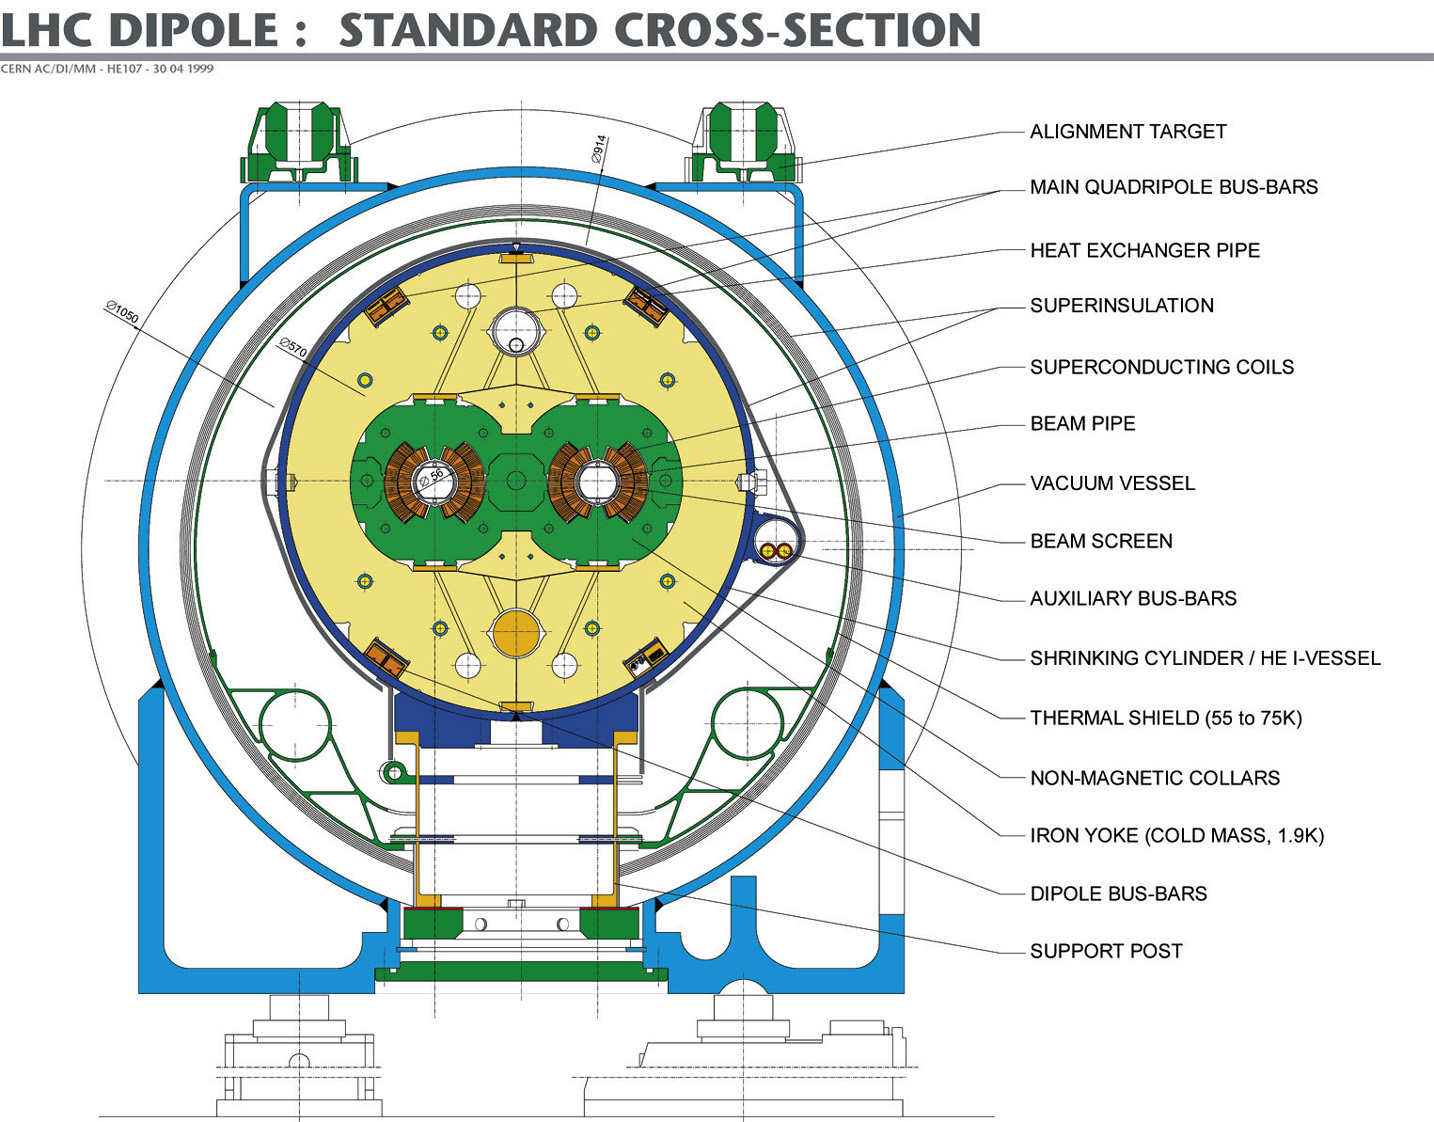
\includegraphics[width=0.9\textwidth]{ATLASLHC/dipole.jpg}
    \caption{
        Diagram showing the cross-section of an \acrshort{LHClabel} dipole magnet~\cite{LHCdipole}. 
    }
    \label{figLHC:dipole}
    \end{center}
\end{figure}

Particles in each beam pipe are accelerated by 8 superconducting \acrlong{RFlabel}~(\acrshort{RFlabel}) cavities, metallic chambers with alternating electric fields housed in cryogenic chambers, which also space the particles into compact groups named bunches. When protons are accelerated, the bunches contain more than $10^{11}$ protons spaced every 25~ns (around 7 meters).\\

The particles are brought to collision at interaction points (IPs) by multiple superconducting magnets focusing the beams. Four detectors are situated at the different IPs: \acrshort{ATLASlabel}, CMS~\cite{CMSmachine}, LHCb~\cite{LHCbmachine} and ALICE~\cite{ALICEmachine}. The first two are multi-purpose experiments that study a wide range of physics, comprising precision measurements of the \acrshort{SMlabel} as well as searches for beyond the SM such as Supersymmetry, exotic particles or dark matter. Both collaborations are formed by around 3000 scientists each, the two largest at \acrshort{CERNlabel}. The LHCb experiment is dedicated to explore hadrons containing $b-$ or $c-$quarks, especially investigating CP-violating processes. The ALICE experiment is the only experiment fully focused on heavy-ion collisions and therefore specialised on QCD physics.\\

The \acrlong{LEPlabel}~(\acrshort{LEPlabel})~\cite{LEPmachine} was the previous main experiment at \acrshort{CERNlabel} and its operations finished in 2000 to start the installation of the \acrshort{LHClabel} in the same tunnel, replacing the predecessor. \acrshort{LEPlabel} was designed to collide $e^+$ and $e^-$ beams and operated at a maximum of $\sqrt{\text{s}}=209$~GeV. Instead, the \acrshort{LHClabel} was designed to accelerate protons or lead ions, which are easier to accelerate to higher energies than eletrons and positrons and provides more collision data, although it is more challenging to study. \acrshort{LEPlabel} explored the \acrshort{EW} scale and provided precision measurements of the \acrshort{SMlabel} setting a lower bound for the mass of the Higgs boson, later discovered using \acrshort{LHClabel} data in 2012. In September 2008, the first \acrshort{LHClabel} operations started and in November 2009 the first collisions were produced. 

\subsection{Performance in Run 2}

The number of events of a certain process is key for its study and can be written as

\begin{equation}
    N = \sigma\mathscr{L} = \sigma \int \mathcal{L} \text{dt},
\end{equation}

where $\sigma$ is the event cross-section for the given process, $\mathscr{L}$ the integrated luminosity and $\mathcal{L}$ the instantaneous luminosity. The cross-section highly depends on the center-of-mass energy $\sqrt{s}$, one of the main characteristics of a particle collider. As a general rule, $\sigma$ increases with $\sqrt{s}$, which is important for~\acrshort{SMlabel} precision measurements or searches for new massive particles.\\

The instantaneous luminosity is another of the main characteristics of a particle collider, and for the \acrshort{LHClabel} can be approximated~\cite{luminosity} to

\begin{equation}
    \mathcal{L} = f \frac{n_1n_2}{4\pi\sigma_x\sigma_y} F,
\end{equation}
%https://cds.cern.ch/record/941318
%https://cds.cern.ch/record/2677054/

with $f$ the revolution frequency, $n_{1,2}$ the total number of protons in each beam and $F$ a reducing factor accounting for the beams not colliding exactly head-on as well as other geometric and beam effects. The first parameter can be approximated to $f=c/27\text{ km} = 11$~kHz and the total number of protons can be inferred from the nominal number of bunches, 2808, which can contain up to $10^{11}$~protons. Finally, the denominator is the approximated transverse beam area with transverse beam size $\sigma_{x,y} = 16.6$~$\mu$m. With these assumptions, the instantaneous luminosity is of $\mathcal{O}(10^{34}$~cm$^{-2}$s$^{-1})$.\\

During 2010 and 2011, the \acrshort{LHClabel} delivered proton collisions at $\sqrt{s}=7$~TeV, and in 2012 at $\sqrt{s}=8$~TeV. The first proton physics run, namely Run~1, ended in February 2013, and were used for the discovery of the Higgs boson. The evolution of the integrated luminosity delivered during Run~2 to the \acrshort{ATLASlabel} experiment is shown in Figure~\ref{figLHC:lumipileup}(a) for a total of $\mathscr{L}=139$~fb$^{-1}$ to be used in physics analysis.\\

Another parameter of interest is the \textit{pile-up}, which is the name given to the additional expected inelastic collisions that occur when crossing bunches of protons. The main source of pile-up interactions are the collisions that appear within a single bunch crossing, called in-time pile-up. In addition, out-of-time pile-up is referred to interactions from neighbouring bunch crossings not resolved fast enough by the detectors. Pile-up effects are a challenge for physics analysis and are inherent to the increase of instantaneous luminosity.\\ %there is a formula

The mean number of interactions per crossing, $\langle\mu\rangle$, is a measure to quantify the pile-up and has changed throughout Run~2, as shown in Figure~\ref{figLHC:lumipileup}(b). Table~\ref{tabLHC:LHCparameters} summarises of some \acrshort{LHClabel} operation parameters during Run~1 and Run~2.

\begin{figure}[htbp]
    \RawFloats
    \begin{center}
    \subfloat[]{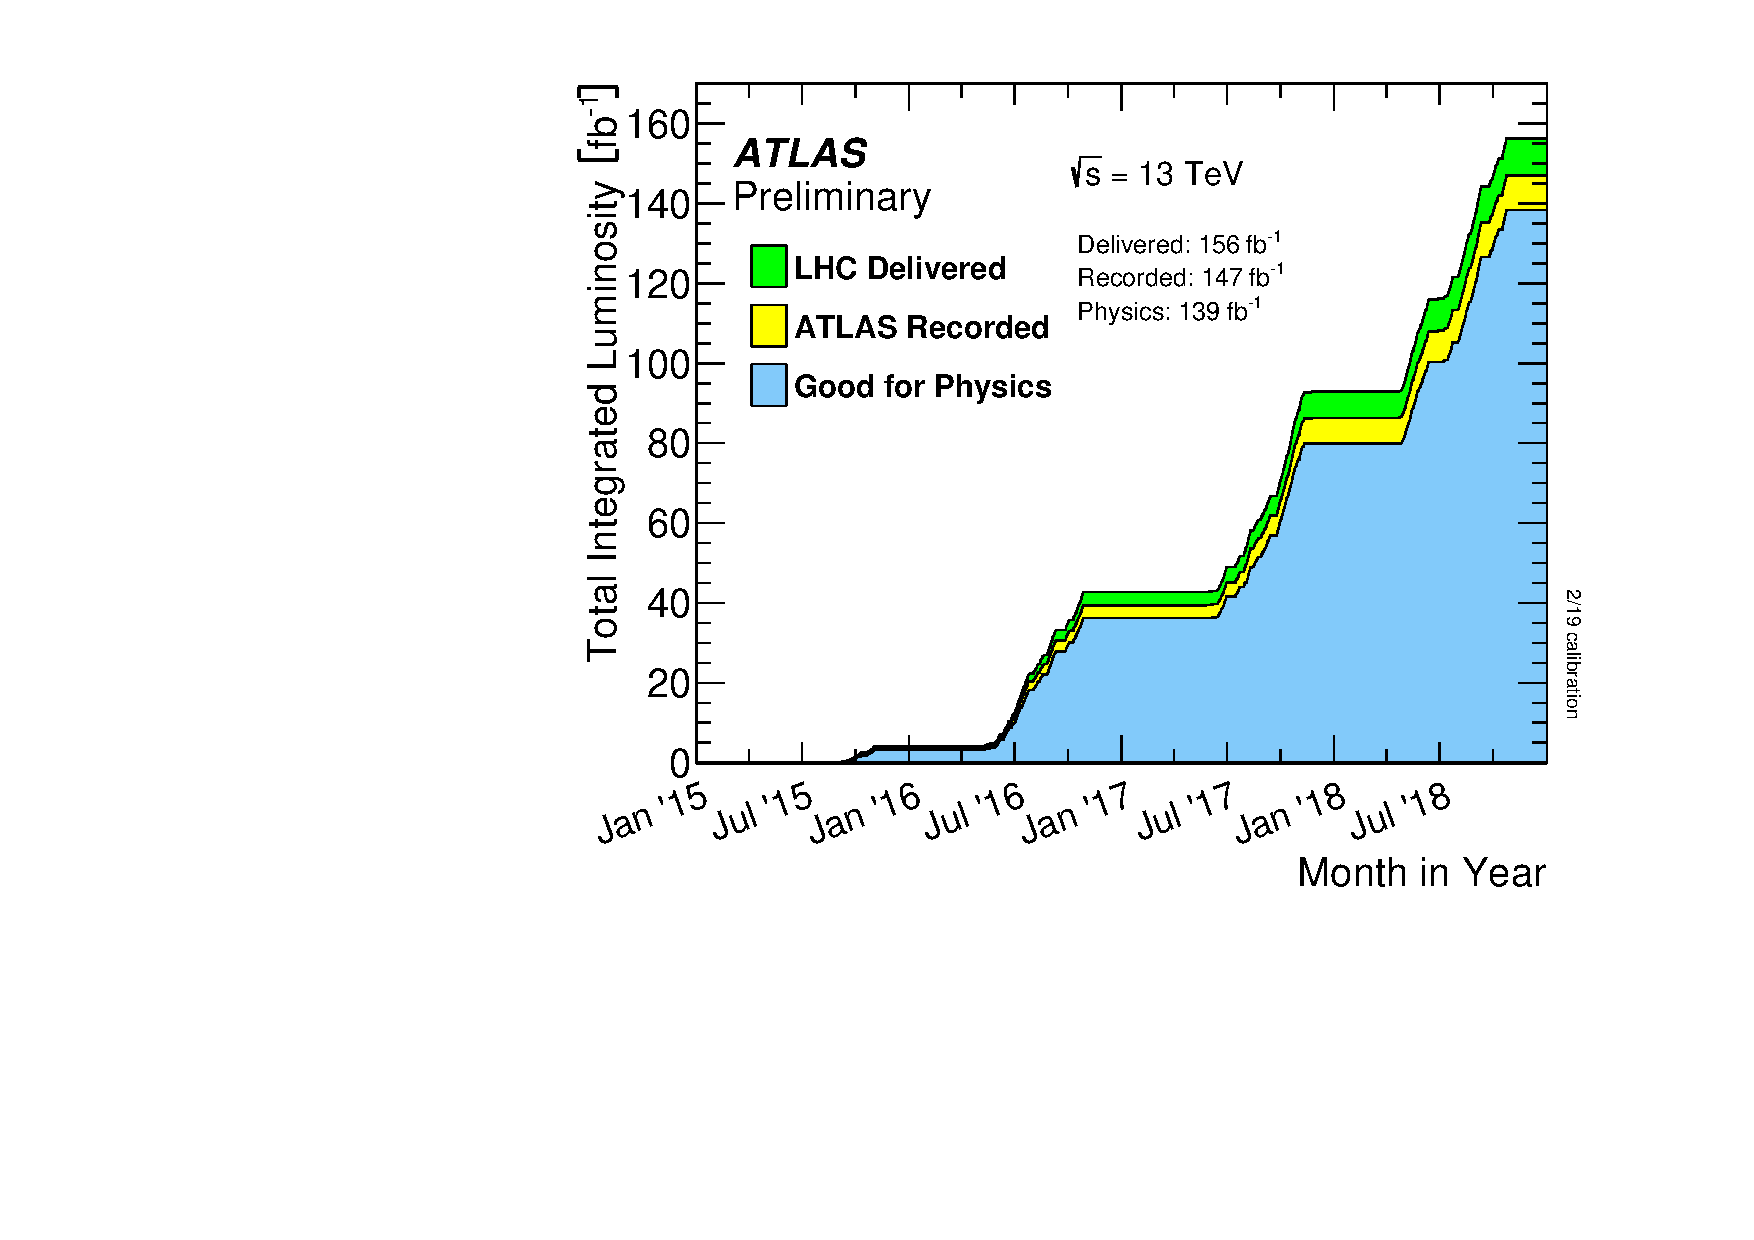
\includegraphics[width=0.47\textwidth]{ATLASLHC/Lumivsyear.pdf}}
    \quad
    \subfloat[]{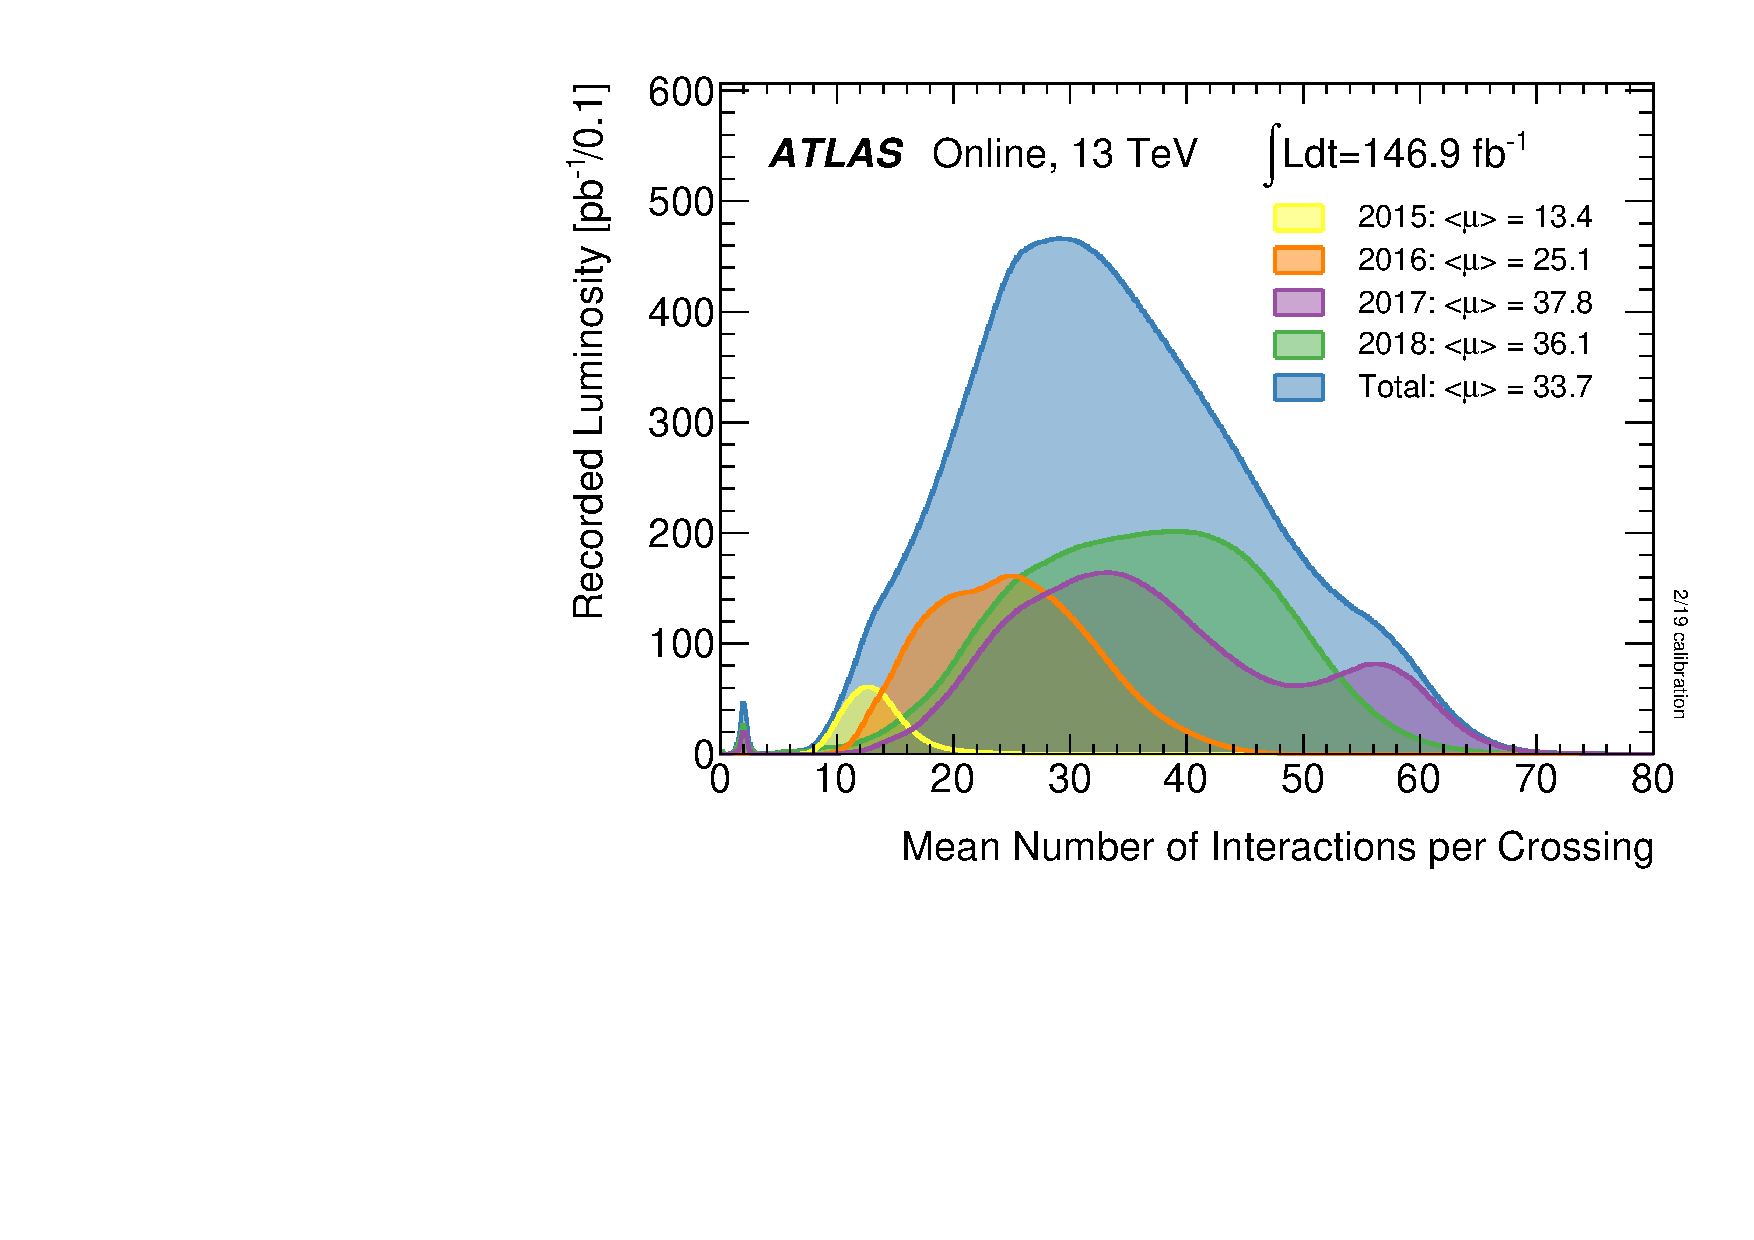
\includegraphics[width=0.47\textwidth]{ATLASLHC/Pileupvsyear.pdf}}
    \caption{
        The total integrated luminosity delivered by the \acrshort{LHClabel}, recorded by \acrshort{ATLASlabel} and labelled good for physics during Run~2 (a) and the mean number of interactions per bunch crossing split into the different data taking periods in Run~2 and weighted by the corresponding luminosity (b)~\cite{publiclumi}. 
    }
    \label{figLHC:lumipileup}
    \end{center}
\end{figure}

\begin{table}[htbp]
    \begin{tabular}{l|ccccccc}
    \toprule\toprule
    Parameter                                        & 2010    & 2011 & 2012 & 2015 & 2016 & 2017 & 2018 \\     \midrule
    Center-of-mass energy [TeV]                                  & 7       & 7    & 8    & 13   & 13   & 13   & 13   \\
    Integrated luminosity (fb$^{-1}$)      & 0.47    & 5.5  & 23   & 4.0  & 38.5 & 50.2 & 63.4 \\
    Peak luminosity [10$^{33}$~cm$^{-2}$s$^{-1}$]     & 0.2     & 3.6  & 7.7  & 5.0  & 13.8 & 20.9 & 21.0 \\
    <Interactions/crossing>                        & $\sim$2 & 9.1  & 20.7 & 13.4 & 25.1 & 37.8 & 36.1 \\
    Bunch spacing [ns]                               & 150     & 50   & 50   & 25   & 25   & 25   & 25   \\
    \bottomrule\bottomrule                               
    \end{tabular}
    \caption{Overview of of the main \acrshort{LHClabel} operational parameters for Run~1 and Run~2 in \acrshort{ATLASlabel}~\cite{publiclumi,publiclumiRun1}.}
    \label{tabLHC:LHCparameters}
    \end{table}

\section{The ATLAS experiment}

The \acrshort{ATLASlabel} detector is a multi-purpose particle detector used to study a wide range of physics topics. It is installed 100~m underground at IP-1 of the \acrshort{LHClabel}. Being 25~m in diameter, 44~m in length and 7000~tonnes in weight, \acrshort{ATLASlabel} is the largest particle detector ever built and installed at a collider. The detector is illustrated in Figure~\ref{figLHC:ATLAS}. It has a cylindrical shape and is composed of several detector layers built around the collision point of the particles, with an almost full solid angle coverage.\\

\begin{figure}[htbp]
    \RawFloats
    \begin{center}
    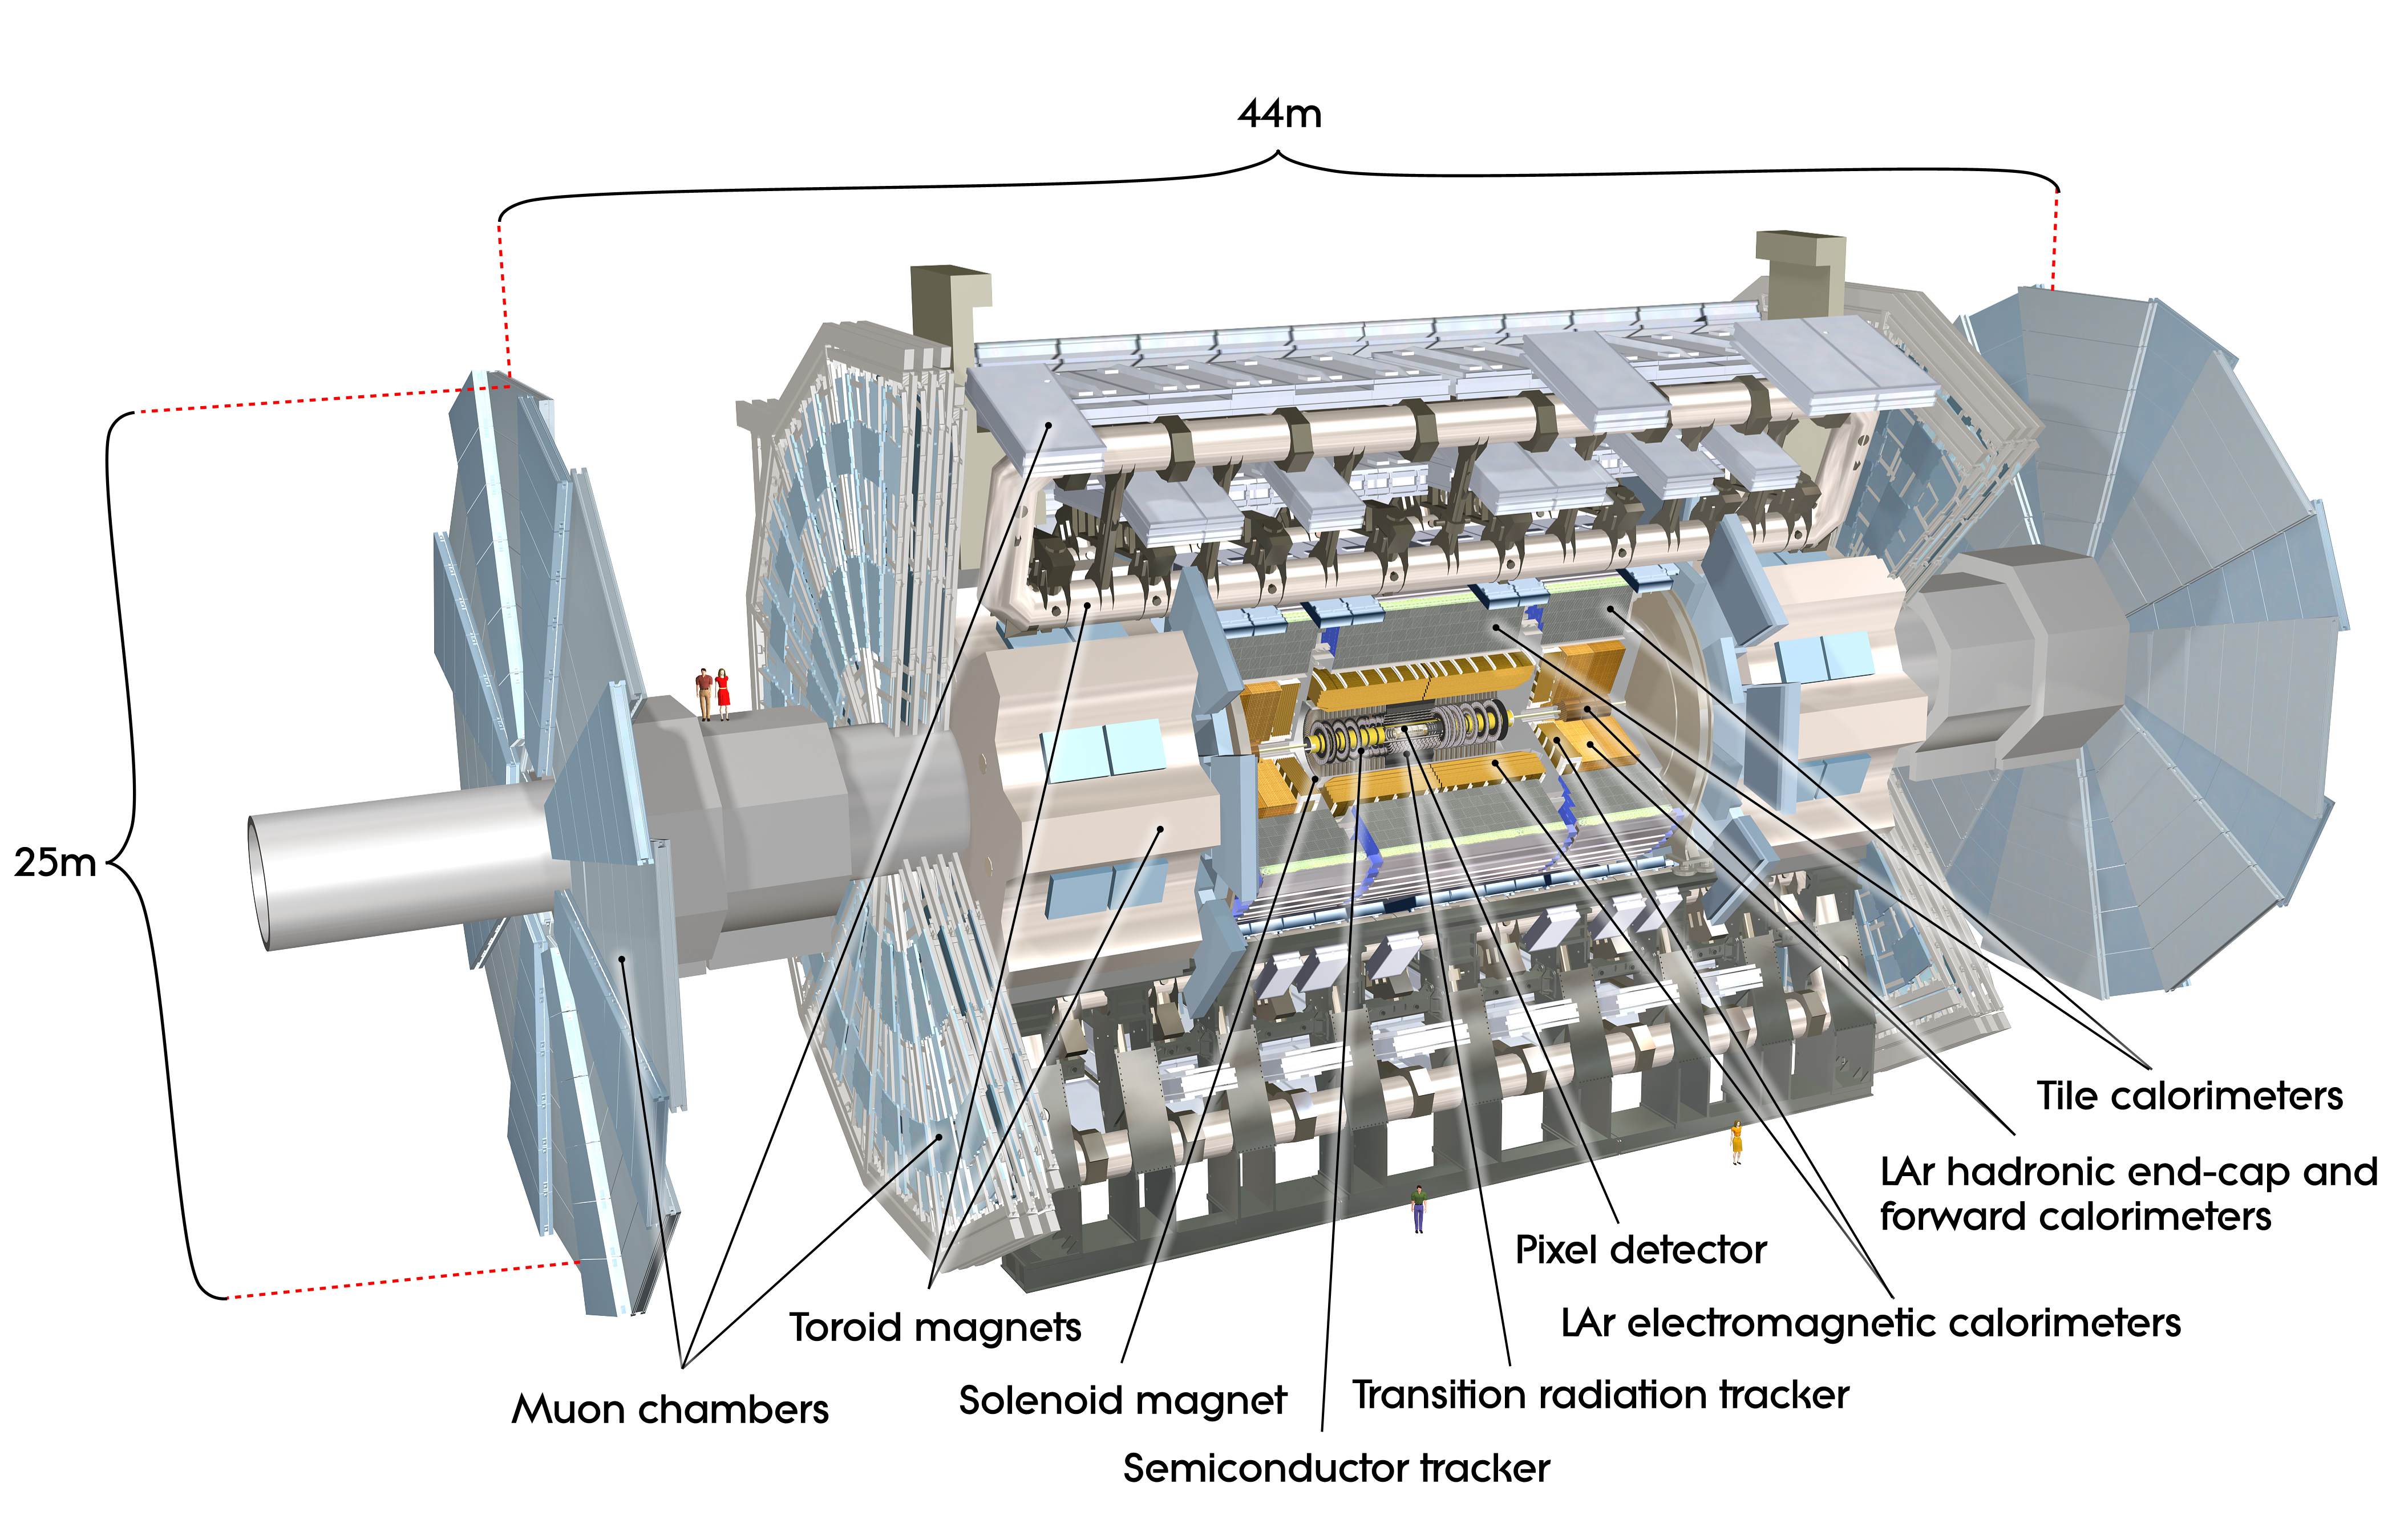
\includegraphics[width=1.0\textwidth]{ATLASLHC/ATLASoverview.jpg}
    \caption{
        Schematic overview of the \acrshort{ATLASlabel} detector~\cite{Collaboration_2008}. 
    }
    \label{figLHC:ATLAS}
    \end{center}
\end{figure}

The data recorded by the detector is used by the collaboration in an extensive physics programme. The luminosity provided by the \acrshort{LHClabel} is large enough to perform both \acrshort{SMlabel} precision measurements and searches for new physics phenomena. The data collected during Run~2 are used to study the Higgs boson and its properties, which has been heavily scrutinised since the first observation of the particle. In addition, measurements of the interactions and processes involving the top-quark are particularly interesting to probe the \acrshort{SMlabel} and \acrshort{BSMlabel} theories. A large portion of the programme is dedicated to a wide range of \acrshort{BSMlabel} theories, which include searches for supersymmetry, dark matter or additional resonances among others. Finally, the physics programme also includes the study of the physics involving $b-$/$c-$quarks as well as heavy ions.\\

All detector systems are designed such that they provide optimal performance to fulfil the physics programme. For that, it is important that the detector can identify particles ranging from few GeV to several TeV with high efficiency and resolution, providing accurate measurements of position and momentum. On the other hand, the electronics have to be highly resistant to radiation and fast to readout to withstand the high energy collisions provided by the \acrshort{LHClabel}.\\

\subsection{Coordinate System}

The convention to describe the particles recorded with the \acrshort{ATLASlabel} detector is a right-handed coordinate system as illustrated in Figure~\ref{figLHC:ATLASframe}, with the origin at the center of the detector which is also the interaction point. The $z$-axis is defined in the counter-clockwise direction along the \acrshort{LHClabel} beam line, the $y$-axis pointing towards the surface and the $x$-axis towards the center of the ring defined by the accelerator. To describe the physics objects within the detector, spherical coordinates are used instead, with the polar angle, $\theta$, measured from the $z$-axis while the azimuthal angle, $\phi$, measured from the $x$-axis in the $x-y$ plane. The pseudorapidity, $\eta$, is usually used instead of the polar angle, as it transforms easily under relativistic boosts along the $z$-axis. For particles with energy $E$ and forward momentum $p_z$, the expression of $\eta$ can be found from the rapidity, $y$, in the high-energy approximation,

\begin{figure}[htbp]
    \RawFloats
    \begin{center}
    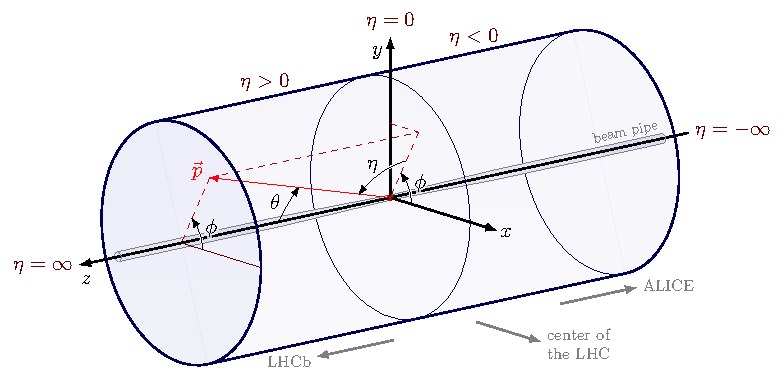
\includegraphics[width=1.0\textwidth]{ATLASLHC/ATLASframe.pdf}
    \caption{
        Schematic overview of the \acrshort{ATLASlabel} coordinate system. 
    }
    \label{figLHC:ATLASframe}
    \end{center}
\end{figure}

\begin{equation}
   y \equiv \frac{1}{2}\ln\left(\frac{E+p_z}{E-p_z}\right) \xrightarrow[ \frac{m}{E} \to 0]{} -\ln\left(\tan\frac{\theta}{2}\right)\equiv \eta
\end{equation}

\acrshort{ATLASlabel} covers the pseudorapidity region up to $|\eta|<4.9$, although physics analyses
typically consider objects restricted to $|\eta|<2.5$. In addition, the difference in $\eta$ between two points, $\Delta\eta$, is invariant under Lorentz transformation, thus angular distances ($\Delta R$) can be described in the $\eta-\phi$ plane as

\begin{equation}
    \Delta R = \sqrt{\left(\Delta\eta\right)^2+\left(\Delta\phi\right)^2},
\end{equation}

with $\Delta\phi$ the difference in $\phi$.

Another useful expression is the momentum in the $x-y$ plane, 

\begin{equation}
    \vec{\pT} = \begin{pmatrix} p_x \\ p_y \end{pmatrix}, \pT = \sqrt{\left(p_x\right)^2+\left(p_y\right)^2}.
\end{equation}

As at the time of the collision the particles are made to collide along the $z$-axis, the initial momentum of the transverse plane is known to be zero due to energy conservation.

\subsection{The Inner Detector}

The \acrlong{IDlabel}~(\acrshort{IDlabel})~\cite{CERN-LHCC-97-016,Haywood:331064,Pixelupgrade} is the innermost detector system, which encloses the beam pipe. This detector system provides precise tracking information of charged particles with momentum as low as 100~MeV with a $|\eta|<2.5$ coverage. Figure~\ref{figLHC:ATLASID} shows an overview of the system, which is structured into three sub-detectors: the pixel detector, the \acrlong{SCTlabel}~(\acrshort{SCTlabel}) and the \acrlong{TRTlabel}~(\acrshort{TRTlabel}).

\begin{figure}[htbp]
    \RawFloats
    \begin{center}
    \subfloat[]{\includegraphics[width=0.47\textwidth]{ATLASLHC/ID_1.jpg}}
    \quad
    \subfloat[]{\includegraphics[width=0.47\textwidth]{ATLASLHC/ID_2.jpg}}
    \caption{
        Schematic view of the \acrshort{ATLASlabel} Inner Detector (a) and details of its barrel section (b)~\cite{Collaboration_2008}. 
    }
    \label{figLHC:ATLASID}
    \end{center}
\end{figure}

\subsubsection*{Pixel Detector}

The innermost part of the \acrshort{IDlabel} is the silicon pixel detector comprising 4 cylindrical layers and 2 end-caps with 3 disc layers each. The layers are located between 33.25~mm to 122.5~mm around the beam pipe with a coverage of $|\eta|$ < 2.5. A single 3D pixel is a radiation-hard silicon detector that produces a small measurable current when a charged particle passes through.\\

The detector is especially important for the reconstruction of tracks, the path followed by charged particles; for the reconstruction of the primary vertex, the position of the main energetic collision; as well as for secondary vertex finding, the position of other concurrent collisions. The \acrlong{IBLlabel}~(\acrshort{IBLlabel})~\cite{Capeans:1291633} is the innermost layer, installed in-between Run~1 and Run~2, having the highest granularity with a pixel size of $50\times 250$~$\mu$m$^2$ (50~$\mu$m in the $\phi$-direction and 250~$\mu$m in the $z$-direction) for a total of 12~M pixels. In particular, the \acrshort{IBLlabel} is very efficient to reconstruct secondary vertices, which are key signatures of long-lived particles decays and crucial for the identification of $b-$hadrons. Furthermore, the three remaining layers have a pixel size of $50\times 400$~$\mu$m$^2$.\\

Overall, the pixel detector contains 86~M pixels with an expected hit resolution of $8\times 40$~$\mu$m$^2$ for the \acrshort{IBLlabel} and $10\times 115$~$\mu$m$^2$ for the rest of pixel layers. In addition, the system makes up around 50\% of all \acrshort{ATLASlabel} readout channels. For the next upgrade, the \acrlong{HLLHClabel}~(\acrshort{HLLHClabel}), a new fully silicon-based \acrlong{ITklabel} Pixel detector~(\acrshort{ITklabel})~\cite{CERN-LHCC-2017-021} will replace the \acrshort{IDlabel}.

\subsubsection*{Semiconductor tracker}

The \acrlong{SCTlabel}~(\acrshort{SCTlabel})~\cite{HABER1998161,SCTperformance} is a silicon strip detector comprising 4 double layers in the barrel region and nine planar end-cap discs on each side, installed around the pixel detector. The planar strips technology is simpler compared to the silicon pixels, for lower resolution covering a larger area. The strips have a size of $80~\mu$m$\times 12$~cm and cover a region up to $|\eta|<2.5$. The two layers within one layer-module are tilted by 40~mrad.\\

Overall, the \acrshort{SCTlabel} has a resolution of $17\times 580$~$\mu$m$^2$ with a total of 6.3~M readout channels. In general, the semiconductor-based detectors in \acrshort{ATLASlabel} operate at a temperature between -10~°C and -5~°C to suppress different types of electronic noise.


\subsubsection*{Transition Radiation Tracker}

The outermost part of the \acrshort{IDlabel} is the \acrlong{TRTlabel}~(\acrshort{TRTlabel})~\cite{MITSOU_2004,TRTRun1}. In contrast to the others, the \acrshort{TRTlabel} is not based on silicon but is a gaseous detector system. It consists of around 300~k straw tubes with a diameter of 4~mm filled with a gas mixture\footnote{In Run~2, a mixture of Ar (80\%) and CO$_2$ (20\%) was used instead in modules with gas leaks} of Xe (70\%), CO$_2$ (27 \%) and O$_2$ (3 \%) and with a gold-plated tungsten wire in the tube center with a potential different to the tube surface of 1.5~kV. When a charged particle hits the tube, the ionisation of the gas is detected as the signal. The straws have a length of 144~cm in the barrel region and 37~cm in the end cap, while the single hit resolution is 120~$\mu$m and 130~$\mu$m, respectively.\\

The \acrshort{TRTlabel} only provides tracking information in the $\phi$ direction, as the tubes are parallel to the beam line. Besides, the \acrshort{TRTlabel} provides particle identification from emitted transition radiation at the material boundaries, since the straws are interleaved with polypropylene. Especially, electrons can be distinguished from charged pions due to larger transition radiation.


\subsection{The Calorimeter System}

The calorimeter system is responsible for the precise measurement of the energy carried by both charged and neutral particles as well as measuring shower properties to allow for particle identification. Showers are cascades of secondary particles which are formed when a highly energetic particle interacts with dense material. \acrshort{ATLASlabel} uses sampling calorimeters which consist of alternating layers of active material (liquid argon and plastic scintillators) and passive detector material (copper, iron, tungsten and lead). While the active material measures the energy deposit of the particles going through, the passive material is designed to interact and absorb particles, thus induces the showering.\\

The calorimeter system covers the region $|\eta|$ < 4.9 and is placed between the central solenoid and the muon spectrometer. Figure~\ref{figLHC:ATLASCalo} shows an overview of the system, which is composed of two sub-detectors: the electromagnetic~\cite{CERN-LHCC-96-041,CERN-LHCC-2017-018} and the hadronic calorimeters~\cite{CERN-LHCC-96-042}. 

\begin{figure}[htbp]
    \RawFloats
    \begin{center}
    \includegraphics[width=1.0\textwidth]{ATLASLHC/Calosystem.jpg}
    \caption{
        Schematic overview of the \acrshort{ATLASlabel} calorimeter system~\cite{Collaboration_2008}. 
    }
    \label{figLHC:ATLASCalo}
    \end{center}
\end{figure}

\subsubsection*{Electromagnetic Calorimeter}

The \acrlong{EMlabel}~(\acrshort{EMlabel}) calorimeter encloses the \acrshort{IDlabel} and is a high granularity calorimeter based on \acrlong{LARlabel}~(\acrshort{LARlabel}) technology with absorber plates made out of lead.\\

To provide full coverage in $\phi$, the \acrshort{EMlabel} calorimeter has an accordion-shaped structure where the active material is placed in the gaps between the lead absorber plates and the Kapton electrodes. The detector operates at -183~°C with a total of 170~k readout channels. The barrel region of the \acrshort{EMlabel} calorimeter covers the region $|\eta|$ < 1.475 and consists of three layers with a 4~mm gap between them and a length of 3.2~m each, with decreasing granularity. The layer closest to the \acrshort{IDlabel} has a granularity of $\Delta\eta\times\Delta\phi= 0.0031\times 0.098$, while the second layer $\Delta\eta\times\Delta\phi= 0.025\times 0.025$ and the outermost $\Delta\eta\times\Delta\phi= 0.05\times 0.025$. In addition, the two end-caps cover the region $|\eta| < 3.2$ with a slightly coarser granularity.\\

In general, the absorption power at high energies of a calorimeter is quantified by means of the radiation length $X_0$ of its medium. It is defined as the distance over which the particle energy is reduced via radiation losses by a factor $1/e$. Given in terms of the radiation length, the thickness of the barrel region is 22 $X_0$ while it is 24 $X_0$ for the end-caps. Moreover, the designed energy resolution~\cite{Collaboration_2008} of the \acrshort{EMlabel} calorimeter is

\begin{equation}
    \frac{\sigma_E}{E} = \frac{10\%}{\sqrt{E}}\oplus\frac{17\%}{E}\oplus 0.7\%.
\end{equation}

\subsubsection*{Hadronic Calorimeter}

The second calorimeter system in \acrshort{ATLASlabel} is the hadronic calorimeter. The system is located around the \acrshort{EMlabel} calorimeter and consists of three components providing around 19~k readout channels. First, the tile calorimeter is made out of alternating layers of steel as absorber material and scintillator plastic tiles as active material, being read out via photomultiplier tubes. The first two layers have the highest granularity with $\Delta\eta\times\Delta\phi= 0.1\times 0.1$. The barrel part of the tile calorimeter covers a region of $|\eta|$ < 1.0 and the two extended barrels the range of 0.8 < $|\eta|$ < 1.7.\\

Next, the end-cap calorimeters are directly outside the \acrshort{EMlabel} calorimeter and are based on the \acrshort{LARlabel} technology. The end-caps use copper as passive material and cover a region of $1.5 < |\eta| < 3.2$ with their highest granularity of also $0.1\times 0.1$ within $|\eta|$ < 2.5. Finally, the forward calorimeter is also \acrshort{LARlabel} based~\cite{Artamonov_2008}, and its first layer uses copper as absorber, which provides information for both electromagnetic and hadronic particles. The other two layers make use of tungsten as absorber, which is better suited for hadronic measurements. In total, the forward calorimeter covers a region of $3.2 < |\eta| < 4.9$.
The designed resolution~\cite{Collaboration_2008} of the tile calorimeter is
\begin{equation}
    \frac{\sigma_E}{E} = \frac{50\%}{\sqrt{E}}\oplus 3\%.
\end{equation}


\subsection{Muon Spectrometer}

The \acrlong{MSlabel}~(\acrshort{MSlabel}) is the outermost detector system of \acrshort{ATLASlabel}, designed to identify muons and measure their energy. Figure~\ref{figLHC:ATLASMuon} shows an overview of the system, which is composed of four detector systems grouped into trigger and precision muon tracking chambers~\cite{CERN-LHCC-97-022,muoncommission}.\\

In total, the \acrshort{MSlabel} has more than one million readout channels and is embedded in three superconducting toroidal magnets, that provide a magnetic field in the $\phi$-direction. Muons mostly reach the \acrshort{MSlabel} without losing energy, and the strong magnetic fields are designed for their precise measurement. The \pT\ resolution is around 3\% for 10-200~GeV and 10\% for 1~TeV muons. 

\begin{figure}[htbp]
    \RawFloats
    \begin{center}
    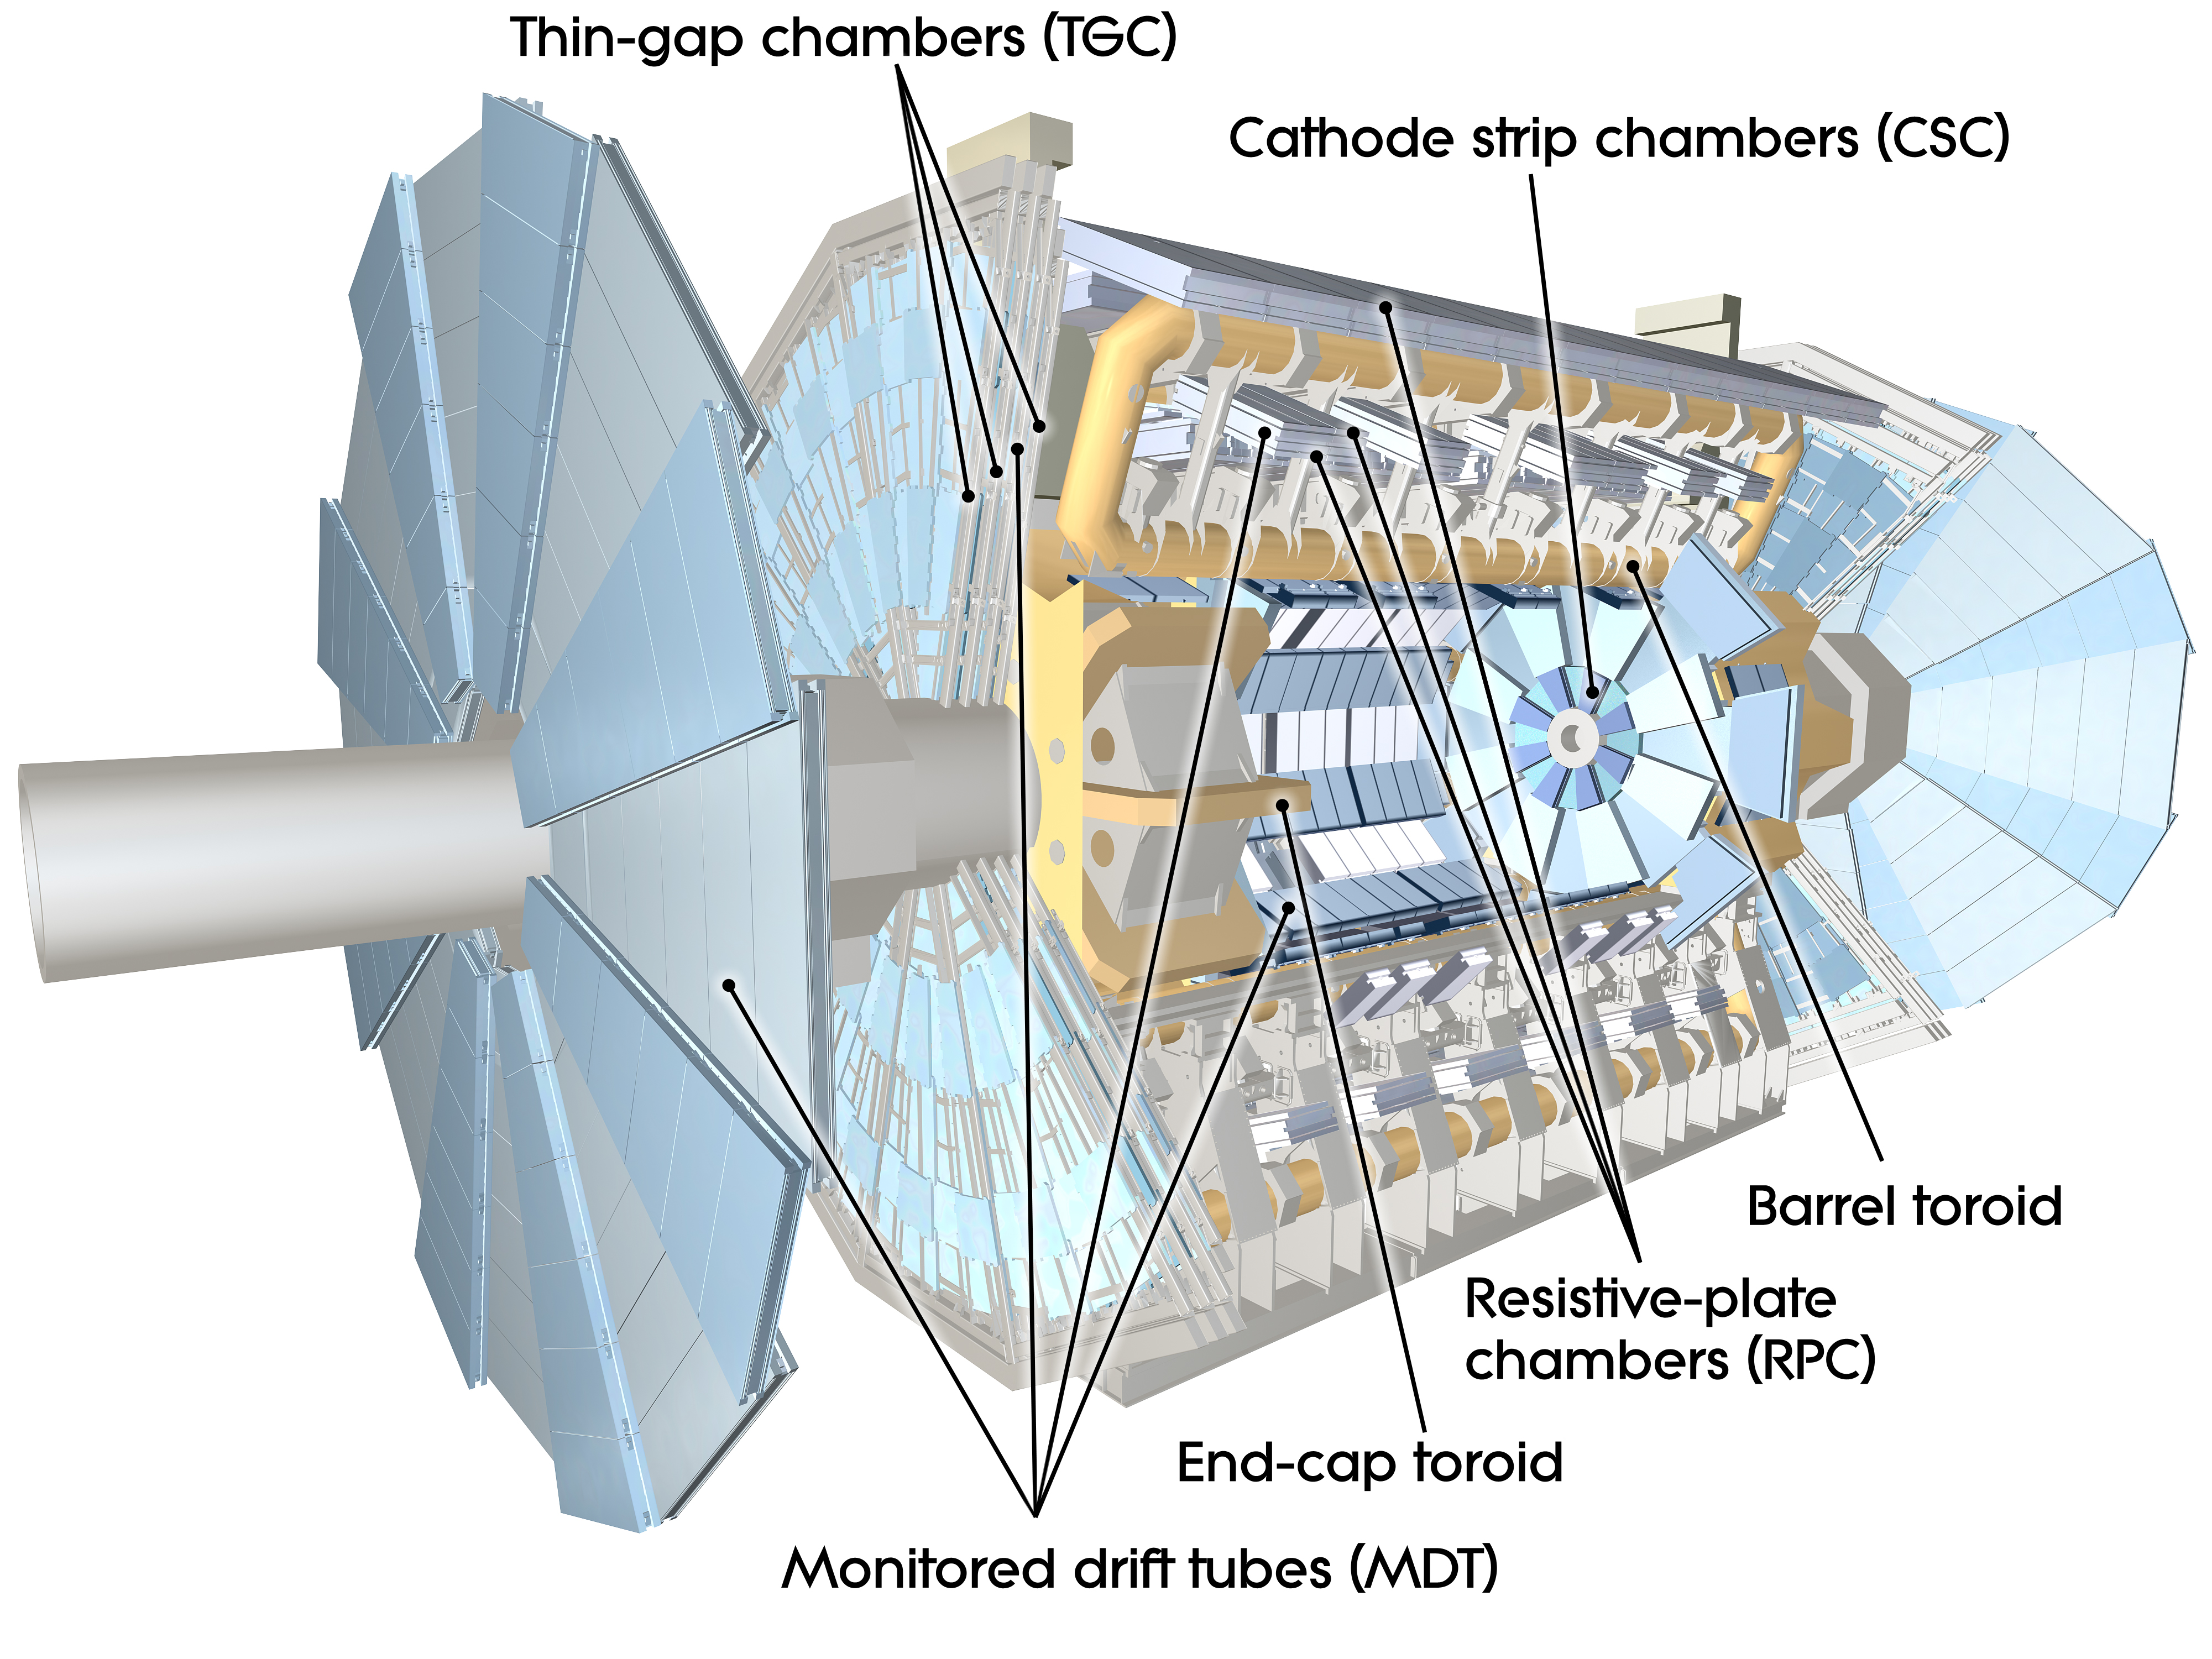
\includegraphics[width=1.0\textwidth]{ATLASLHC/Muonsystem.jpg}
    \caption{
        Schematic overview of the \acrshort{ATLASlabel} muon spectrometer~\cite{Collaboration_2008}. 
    }
    \label{figLHC:ATLASMuon}
    \end{center}
\end{figure}

\subsubsection*{Muon Trigger Chambers}

The muon trigger chambers are designed for a fast readout to provide energetic muon identification in a timescale compatible with every bunch crossing. In the barrel region, $|\eta|$ < 1.05, three layers of \acrlong{RPClabel}~(\acrshort{RPClabel}) consistsing of two parallel plates with high resistivity and filled with a gas mixture (94.7\% C$_2$H$_2$F$_4$, 5\% Iso-C$_4$H$_{10}$, 0.3\% SF$_6$) are installed.\\

The \acrshort{RPClabel} provide an $\eta-\phi$ measurement with a spatial resolution of 10~mm and time resolution of 1.5~ns. \acrlong{TGClabel}~(\acrshort{TGClabel}) are installed in the end-caps, $1.05 < |\eta| < 2.4$, and consist of multi-wire chambers filled with a gas mixture (55\% CO$_2$ and 45\% n-C$_5$H$_{12}$) with the wires separated by 1.8~mm. Besides trigger information, the \acrshort{TGClabel} provide $\phi$ information with a resolution of 5~mm.

\subsubsection*{Precision Muon Tracking Chambers}

The precision muon tracking chambers are designed to provide high resolution and precision tracking information. The system is mainly composed of \acrlong{MDTlabel}~(\acrshort{MDTlabel}), installed in the barrel and end-cap region covering $|\eta|$ < 2.7. \acrshort{MDTlabel} are aluminium drift tubes with 3~cm of diameter filled with a gas mixture (95\% Ar and 7\% \ensuremath{\mathrm{CO_2}}). Each chamber contains 3-8 layers of drift tubes with a spatial resolution of 35~$\mu$m.\\

The forward region of the system, 2.0 < $|\eta|$ < 2.7, is covered by \acrlong{CSClabel}~(\acrshort{CSClabel}) and provide a resolution of 40~$\mu$m in the radial direction and 5~mm in the $\phi$ direction~\cite{Collaboration_2008}. These chambers are proportional multi-wire chambers, similar to the \acrshort{TGClabel}, with lower response time.

\subsection{Magnet System}

The magnet system is of major importance to allow momenta and charge measurements, bending the trajectory of charged particles depending on these properties. Figure~\ref{figLHC:ATLASMagnets} shows an overview of the system, which consists of two sub-systems: the central solenoid magnet, located between the \acrshort{IDlabel} and the calorimeters, and the toroidal magnet system, embedded within the \acrshort{MSlabel}.\\

The solenoid generates a constant magnetic field of 2~T, with a superconducting magnet made out of NbTi cooled via liquid helium to a temperature of 1.8~K. There is one barrel toroid magnet and two end-cap toroid magnets with eight coils each, each delivering an inhomogeneous magnetic field of roughly 0.5~T and 1~T, respectively.

\begin{figure}[htbp]
    \RawFloats
    \begin{center}
    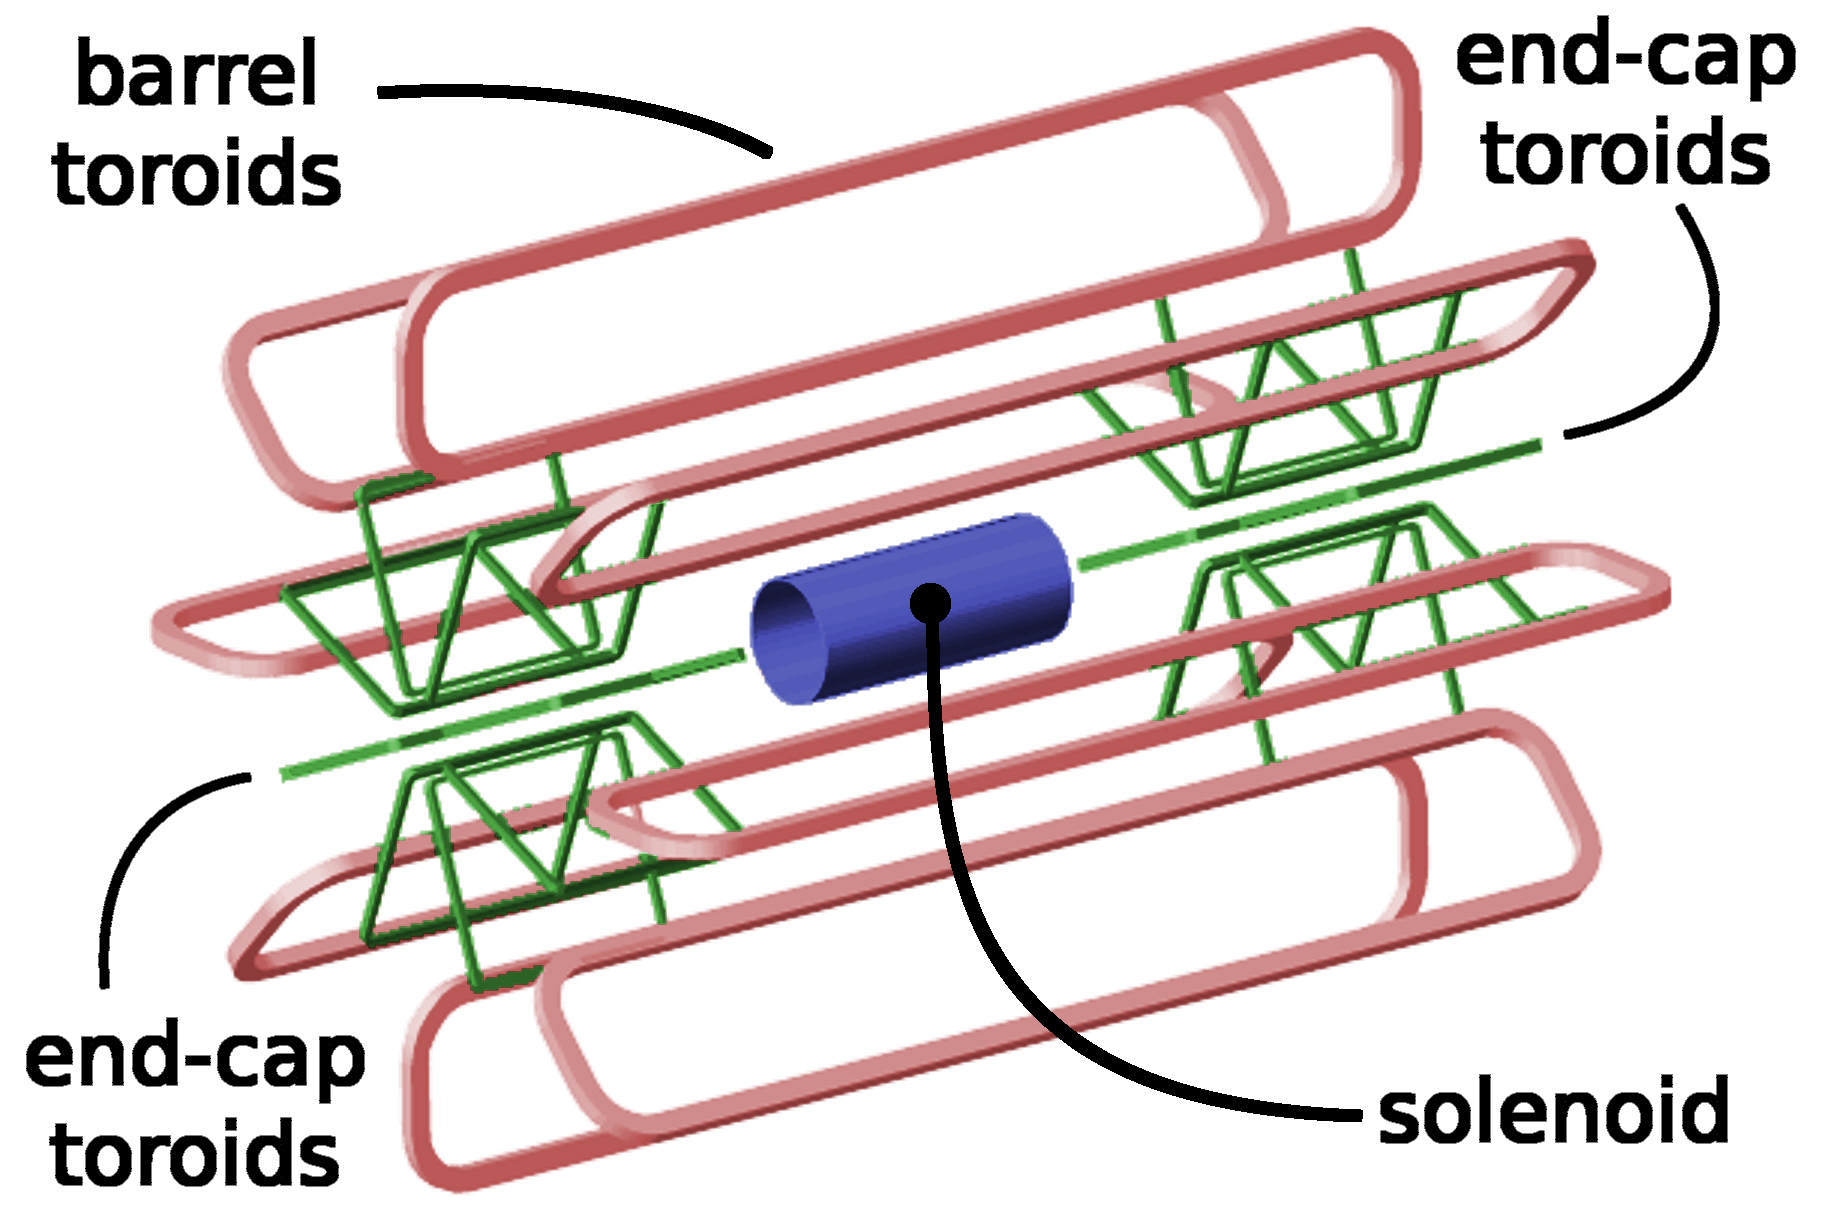
\includegraphics[width=0.8\textwidth]{ATLASLHC/magnetSystems.png}
    \caption{
        Schematic overview of the \acrshort{ATLASlabel} magnet system~\cite{JetGoodson}. 
    }
    \label{figLHC:ATLASMagnets}
    \end{center}
\end{figure}

\subsection{Trigger System and Data Acquisition}

With bunches crossing every 25~ns, the \acrshort{LHClabel} produces collisions at a frequency of 40~MHz at nominal operation conditions. For \acrshort{ATLASlabel}, this is translated to an unmanageable rate of more than 60~TB/s of data. The \acrlong{TDAQlabel}~(\acrshort{TDAQlabel}) system is designed to select and record the events considered interesting for analysis for an average storage rate of 1~kHz.\\

The trigger system is structured into two parts since Run~II~\cite{Jenni:616089,Ruiz-Martinez:2133909}: the \acrlong{L1label}~(\acrshort{L1label}) hardware-based trigger system and the software-based \acrlong{HLTlabel}~(\acrshort{HLTlabel}). The \acrshort{L1label} trigger uses reduced granularity information from the calorimeters and from the muon \acrshort{RPClabel} and \acrshort{TGClabel} to select events with interesting signatures (normally corresponding to high \pT\ electrons, muons, photons, jets or high missing transverse momentum). The \acrshort{L1label} system reduces the rate from 40~MHz to about 100 kHz with a computing time (or latency) of 2.5~$\mu$s. The information of the collisions is stored in buffers and the \acrlong{CTPlabel}~(\acrshort{CTPlabel}) performs the decision based on the inputs of the various \acrshort{L1label} sub-systems. The \acrshort{L1label} trigger output consists of \acrlong{RoIlabel}~(\acrshort{RoIlabel}) in $\eta$ and $\phi$, and are sent to the \acrshort{HLTlabel}. The \acrshort{HLTlabel} uses the full detector information within the \acrshort{RoIlabel} to reduce the event rate down to approximately 1~kHz with a latency of 200~ms. A schematic of the~\acrshort{ATLASlabel} trigger system is presented in Figure~\ref{figLHC:ATLASTDAQ}.\\

After, the data is transferred to a computing center for further processing and storage. An offline data quality monitoring system performs checks on fully reconstructed events, to ensure their quality for use in physics analyses. Validation criteria include requirements on the condition and performance of the beams and different \acrshort{ATLASlabel} sub-detectors at the time of operation. As displayed in Figure~\ref{figLHC:lumipileup}(b), from the 156~fb$^{-1}$ of integrated luminosity delivered by the \acrshort{LHClabel} during Run~2, 147~fb$^{-1}$ were recorded by the detector and 139~fb$^{-1}$ catalogued as good-quality data.

\begin{figure}[htbp]
    \RawFloats
    \begin{center}
    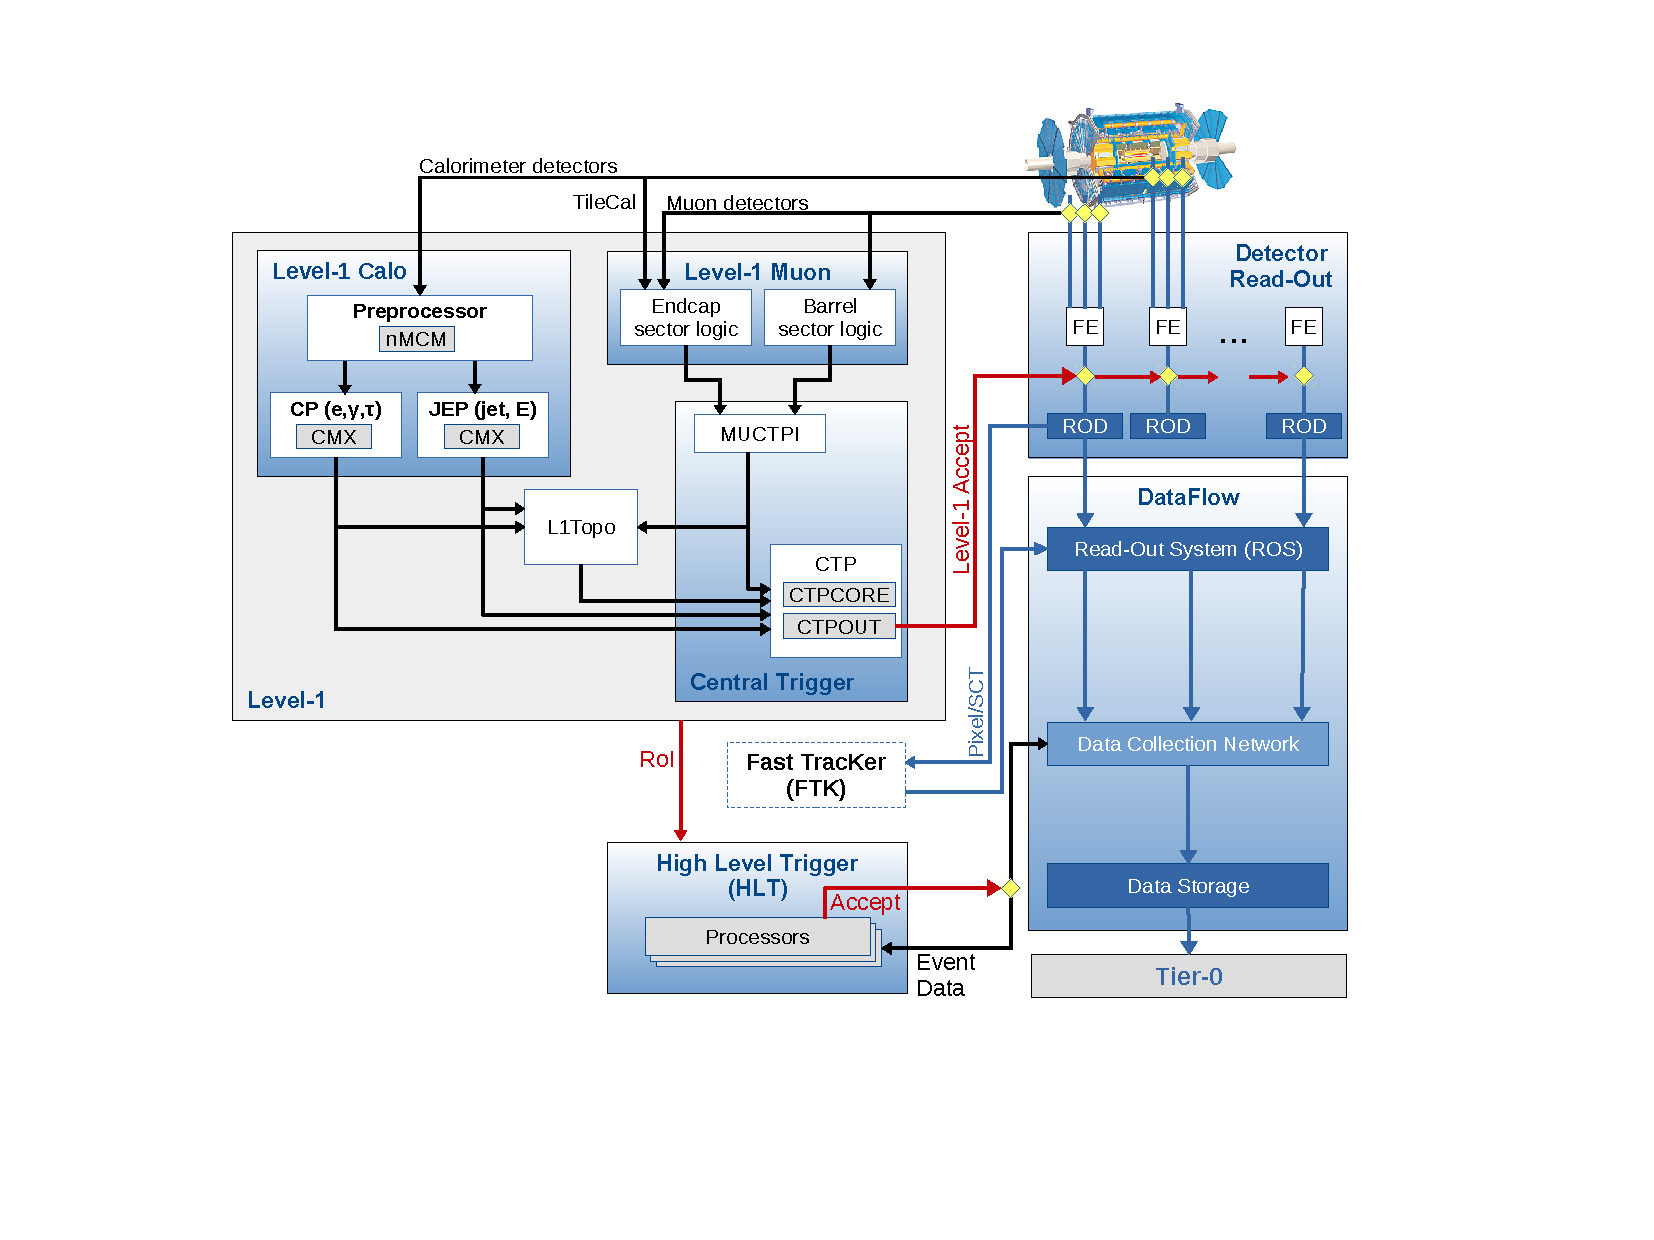
\includegraphics[width=1.0\textwidth]{ATLASLHC/Triggerscheme.pdf}
    \caption{
        Schematic overview of the \acrshort{ATLASlabel} Trigger and Data Acquisition system in Run~2~\cite{publicTDAQ}. 
    }
    \label{figLHC:ATLASTDAQ}
    \end{center}
\end{figure}